\section{Experimental Evaluation}
\label{sec:evaluation}

In this section, we evaluate all implemented algorithms extensively and report on the insights gained. For this section, the algorithm from \citeauthor{on_optimal_polyline_simplification_using_the_hausdorff_and_frechet_distance} will be referred to as the \emph{simple algorithm}, while the algorithm from \citeauthor{polyline_simplification_has_cubic_complexity_bringmannetal} will be referred to as the \emph{advanced algorithm}.

\subsection{Data and Hardware}
\label{subsec:hardware}

\subsubsection{Software and Data}
\label{subsubsec:software}

All algorithms were implemented in C++ and compiled using GCC with the -O3 flag for compiler optimizations and the -flto flag for link-time optimizations. The simple algorithms were parallelized using OpenMP with dynamic scheduling and a chunk size of 32 over the two nested loops iterating over \(i\) and \(j\).

The polylines used in the test cases were automatically generated using a variety of parameters. These include the minimum and maximum allowed length for each line segment of the polyline, as well as the maximum angle that a line segment is allowed to deviate from the previous one. For example, a maximum angle of zero degrees generates polylines that are effectively straight lines, while a maximum angle of \(180^\circ\) allows for arbitrarily shaped polylines. The reasoning is that small angles force the polyline to be smoother, while larger angles cause more erratic and less well-behaved polylines. We test both well-behaved polylines (maximum angle \(60^\circ\)) and non-well-behaved polylines (maximum angle \(180^\circ\)).

The minimum and maximum line segment lengths were fixed to 2 and 10 units, respectively. The exact value for the maximum length is arbitrary, as any polyline can be scaled accordingly, and the results scale with \(\varepsilon\). The minimum line segment length of 2 was enforced for three primary reasons:
\begin{itemize}
	\item To prevent the simulation of arbitrary angles through chains of very short line segments.
	\item To reduce the variance in line segment lengths, improving the clarity of visualizations.
	\item To mitigate numerical instability and avoid divisions by zero that could occur with zero-length segments, which our algorithms do not explicitly handle.
\end{itemize}

To generate the polylines, we fix the first point at the origin (since simplifications are invariant under translation) and sample an initial direction uniformly at random. We then iteratively sample a line segment length and a deviation angle, which is added to the current direction. Each deviation angle is chosen uniformly from \([-\alpha, \alpha]\), where \(\alpha\) is the maximum angle. The line segment length is not chosen uniformly; instead, to sample the next point uniformly from the annular sector defined by the maximum angle and the length bounds, we use inverse transform sampling. This results in choosing the length as \(\sqrt[d]{m^d + (M^d - m^d)U}\), where \(d\) is the dimension, \(m\) and \(M\) are the minimum and maximum lengths, and \(U\) is a uniform random variable on \([0,1]\). This generation method works in arbitrary dimensions, but we restrict ourselves to two dimensions, as that is the most relevant use case and can be visualized easily.

Examples of such generated polylines can be seen in \cref{fig:well-behaved-300} and \cref{fig:non-well-behaved-300}.

\begin{figure}[b]
  \centering
  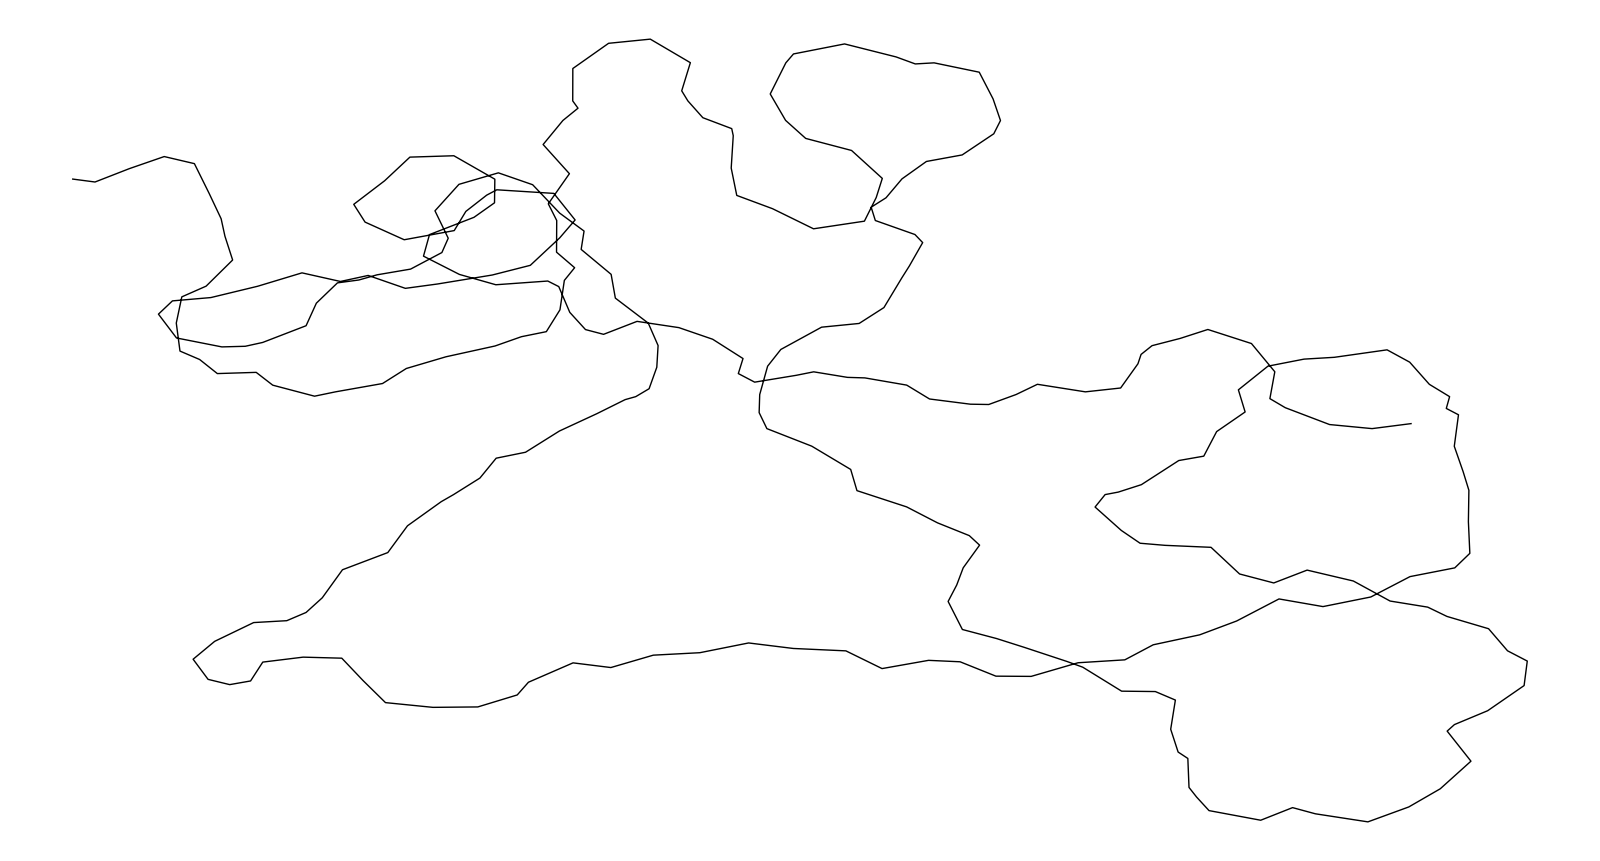
\includegraphics[scale=0.3]{./figures/well-behaved-300.png}
  \caption{Example of a well-behaved polyline consisting of \(300\) points in \(2\) dimensions.}
  \label{fig:well-behaved-300}
\end{figure}

\begin{figure}[b]
  \centering
	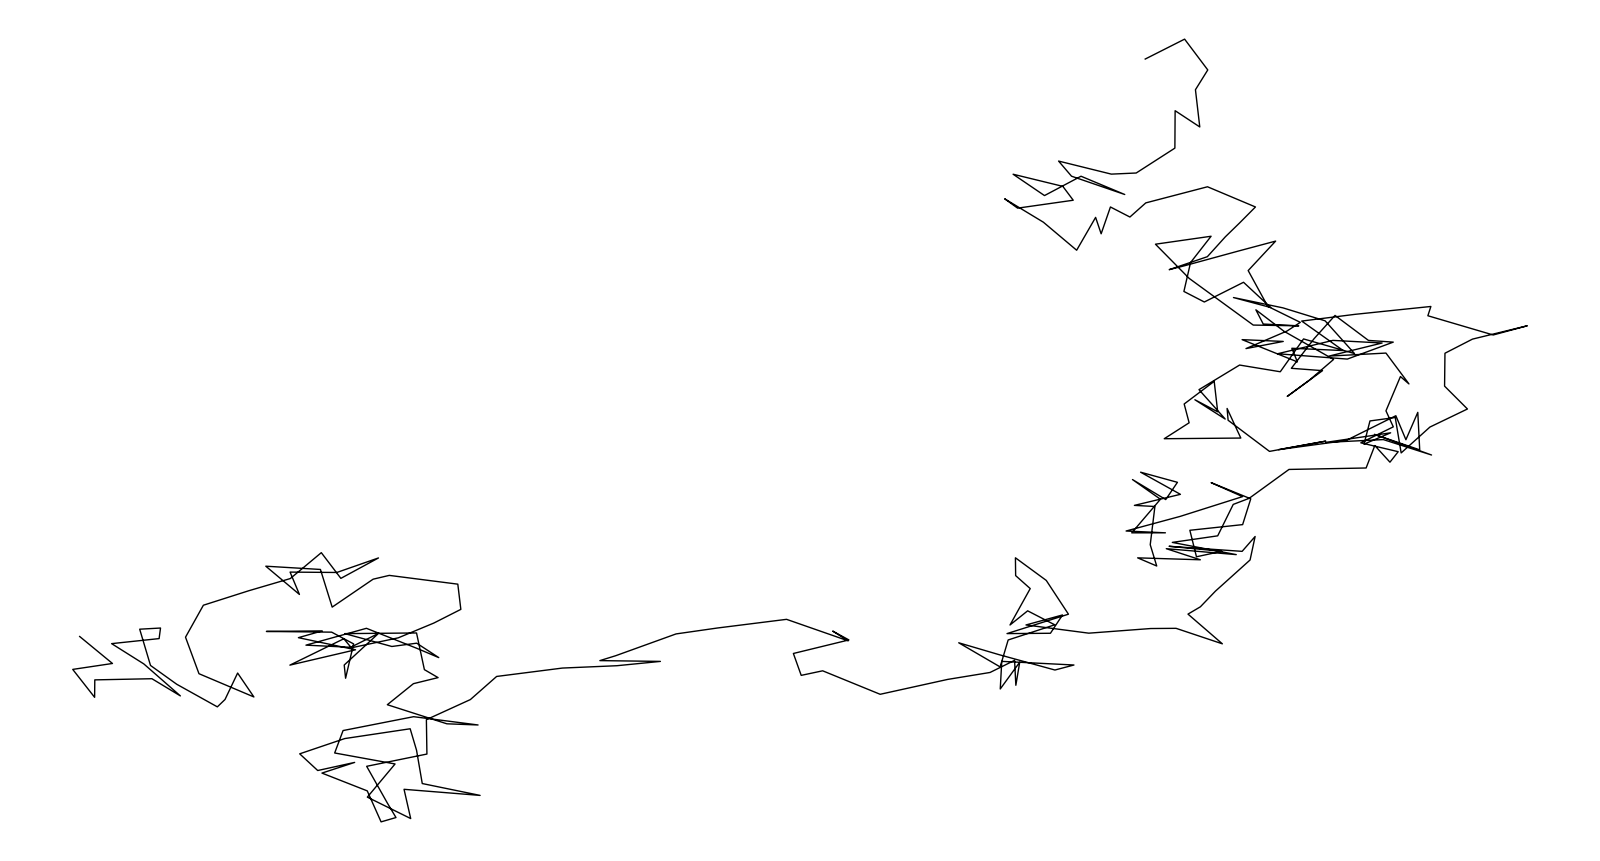
\includegraphics[scale=0.3]{./figures/non-well-behaved-300.png}
  \caption{Example of a non-well-behaved polyline consisting of \(300\) points in \(2\) dimensions.}
  \label{fig:non-well-behaved-300}
\end{figure}

\subsubsection{Hardware}
\label{subsubsec:hardware}
The experiments were conducted on a system with an AMD Ryzen 5 7520U CPU (4.38 GHz, 8 cores) running Arch Linux.

\subsection{Experimental Setup}
\label{subsec:exp_setup}

We test the following nine variants:
\begin{itemize}
	\item Simple Euclidean Algorithm
	\item Simple Manhattan Algorithm
	\item Simple Chebyshev Algorithm
	\item Simple Implicit Euclidean Algorithm
	\item Simple Semiexplicit Euclidean Algorithm
	\item Advanced Euclidean Algorithm
	\item Advanced Manhattan Algorithm
	\item Advanced Chebyshev Algorithm
	\item Advanced Semiexplicit Euclidean Algorithm
\end{itemize}

We have not implemented an implicit version of the advanced algorithm, as it would require a complete rewrite of the complex \citeauthor{polyline_simplification_has_cubic_complexity_bringmannetal} algorithm and its dependencies. All non-implicit variants (including the semiexplicit ones) can be implemented as a single algorithm where the necessary changes are abstracted using C++ templates to reduce code duplication.

Due to the extensive parameter space, a comprehensive evaluation of every possibility is infeasible. We thus must select specific criteria to test. We encourage the interested reader to experiment with different variations, as we observed that even minor changes can lead to different results.

Notably, during preliminary testing, five of the nine main algorithms proved to be the fastest under different conditions (e.g., compiler flags, input size), highlighting the high dependency of performance on the experimental environment. The specific variants were:
\begin{itemize}
	\item Simple Implicit Euclidean in a concurrent setting on small polylines
	\item Simple Chebyshev under parallel execution without link-time optimization on small polylines
	\item Advanced Chebyshev without link-time optimization on long polylines
	\item Simple Euclidean under parallel execution with link-time optimization on small polylines
	\item Advanced Euclidean with link-time optimization on long polylines
\end{itemize}
Note that this does not mean these conditions were optimal for the individual algorithms, but rather reflects their speed relative to the other variants under those specific settings.

We list our main experimental choices below. Many effects on runtime may be implementation-, hardware-, or even operating system-specific, so we cannot guarantee the same results elsewhere.

\begin{itemize}
	\item \textbf{Compiler optimizations (-O3):} This generally resulted in a performance boost by a factor of approximately \(10\) for all variants. There was no reason to test without optimizations.
	\item \textbf{Link-time optimizations (-flto):} For most variants, enabling this flag resulted in a \(20\%\) performance boost. The only exception was the semiexplicit version of the simple algorithm, which was noticeably slower for unknown reasons.
	\item \textbf{Polyline types:} We test on both well-behaved (max angle \(60^\circ\)) and non-well-behaved (max angle \(180^\circ\)) polylines. Line segment lengths are restricted to \([2, 10]\).
	\item \textbf{Choice of \(\varepsilon\):} We generally set \(\varepsilon = 2\) unless stated otherwise. This value was chosen because \(\varepsilon^2 \neq \varepsilon\), which helped detect mistakes in the semiexplicit implementations (which use \(\varepsilon^2\) internally but must yield the same result as the explicit version). This choice affects the simplification size and thus the runtime of the simple algorithms, but not the advanced algorithms.
	\item \textbf{Implementation details:} We observed that seemingly minor details, such as function inlining, could affect runtime by up to \(20\%\). We tried to select the best-performing versions, but it is likely that even better choices exist depending on the compiler and hardware.
\end{itemize}

\subsection{Optimization Tests}
Before presenting the main results, we explore the effects of the optimizations from \cref{ssec:optimizations} applied to the simple algorithm. In the following sections, we will use all optimizations for further comparisons.

We test the following optimizations:
\begin{itemize}
	\item Parallelization (p)
	\item Reachability optimization (r)
	\item Local minimality optimization (l)
	\item Global minimality optimization (g)
\end{itemize}

For parallelization, we compare the fully parallelized version (8 cores) against the sequential version. For the other three, we test the algorithm with and without each optimization. We also test the algorithm with no optimizations applied. All tests use well-behaved data and average over 20 test cases per point count, for polylines up to length 200.

First, we compare the effect of parallelization. \Cref{fig:simple-seq} shows both the sequential and parallelized versions. The parallelized versions are consistently about three times faster.

\begin{figure}[b]
  \centering
	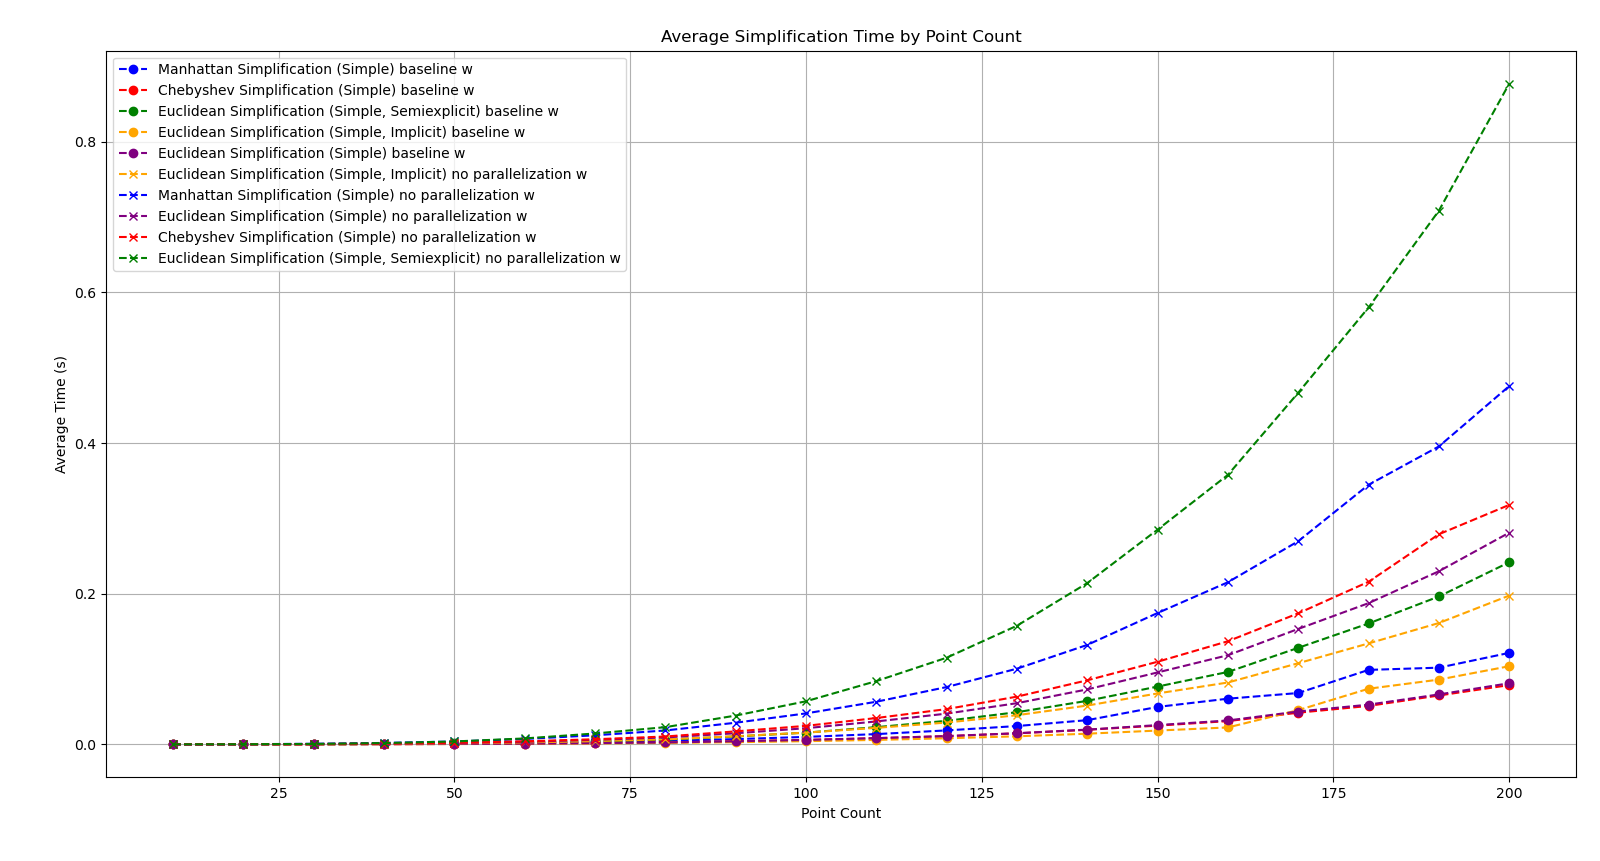
\includegraphics[scale=0.4]{./figures/simple-seq.png}
  \caption{Simple algorithm with and without parallelization.}
  \label{fig:simple-seq}
\end{figure}

Next, we inspect how the other optimizations affect runtime. All following tests are parallelized. \Cref{fig:simple-noopt} compares having all three optimizations versus having none of them. Without any optimizations, the theoretical \(\Oh(n^6)\) runtime seems to be evident. The figure illustrates the significant effectiveness of these optimizations.

\begin{figure}[b]
  \centering
	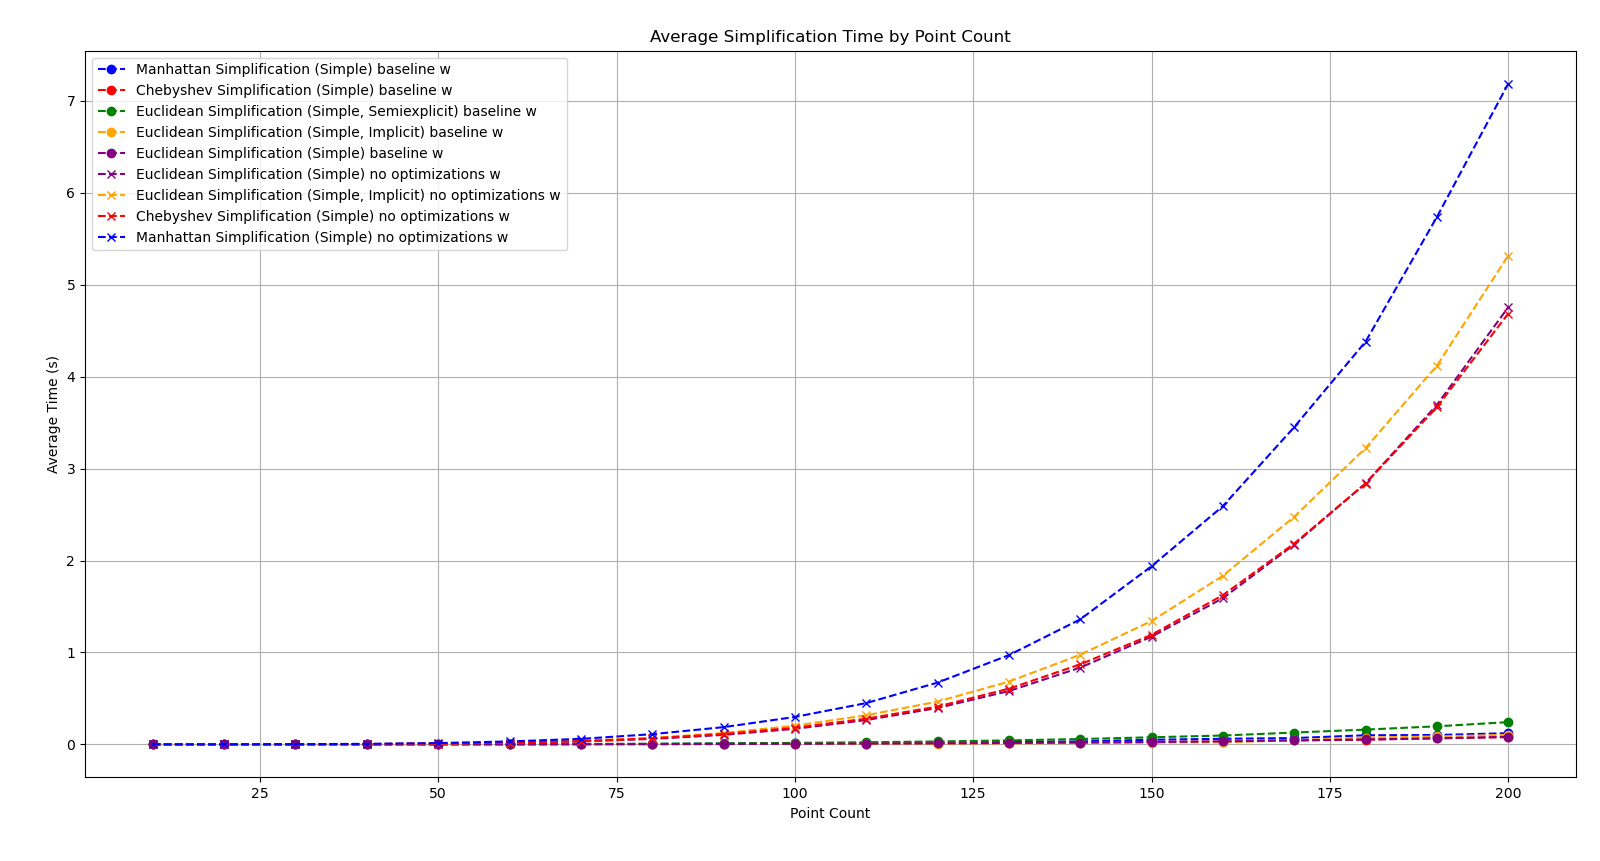
\includegraphics[scale=0.4]{./figures/simple-noopt.png}
  \caption{Simple algorithm with all optimizations and with none of them.}
  \label{fig:simple-noopt}
\end{figure}

Finally, we compare the effect of omitting exactly one of the three optimizations. \Cref{fig:simple-g} omits the global optimality optimization, \cref{fig:simple-l} omits the local optimality optimization, and \cref{fig:simple-r} omits the reachability optimization.

The reachability optimization has little effect on most variants but a massive one on the implicit variant. We have no definitive explanation for this, as the main logic should be the same for all variants.

The local minimality optimization also has almost no effect on most variants, with the noticeable exceptions being the implicit variant and a slight but consistent improvement in the Manhattan variant.

The global minimality optimization has the most positive effect. Note that \cref{fig:simple-g,fig:simple-l,fig:simple-r} each show performance with two optimizations enabled, omitting one. The performance improvements seen in these figures do not add up to the total improvement seen in \cref{fig:simple-noopt}, suggesting that the optimizations have significant overlap in the parts of the algorithm they speed up. This can be explained, particularly for the local and global minimality optimizations: if the local optimization is triggered in a layer, the global optimization will be triggered in all subsequent layers for the same cell entry, explaining why the global optimization appears more beneficial.

For the main results, we use all optimizations and parallelization, as they have proven to be beneficial, especially for the implicit variant.

\begin{figure}[b]
  \centering
	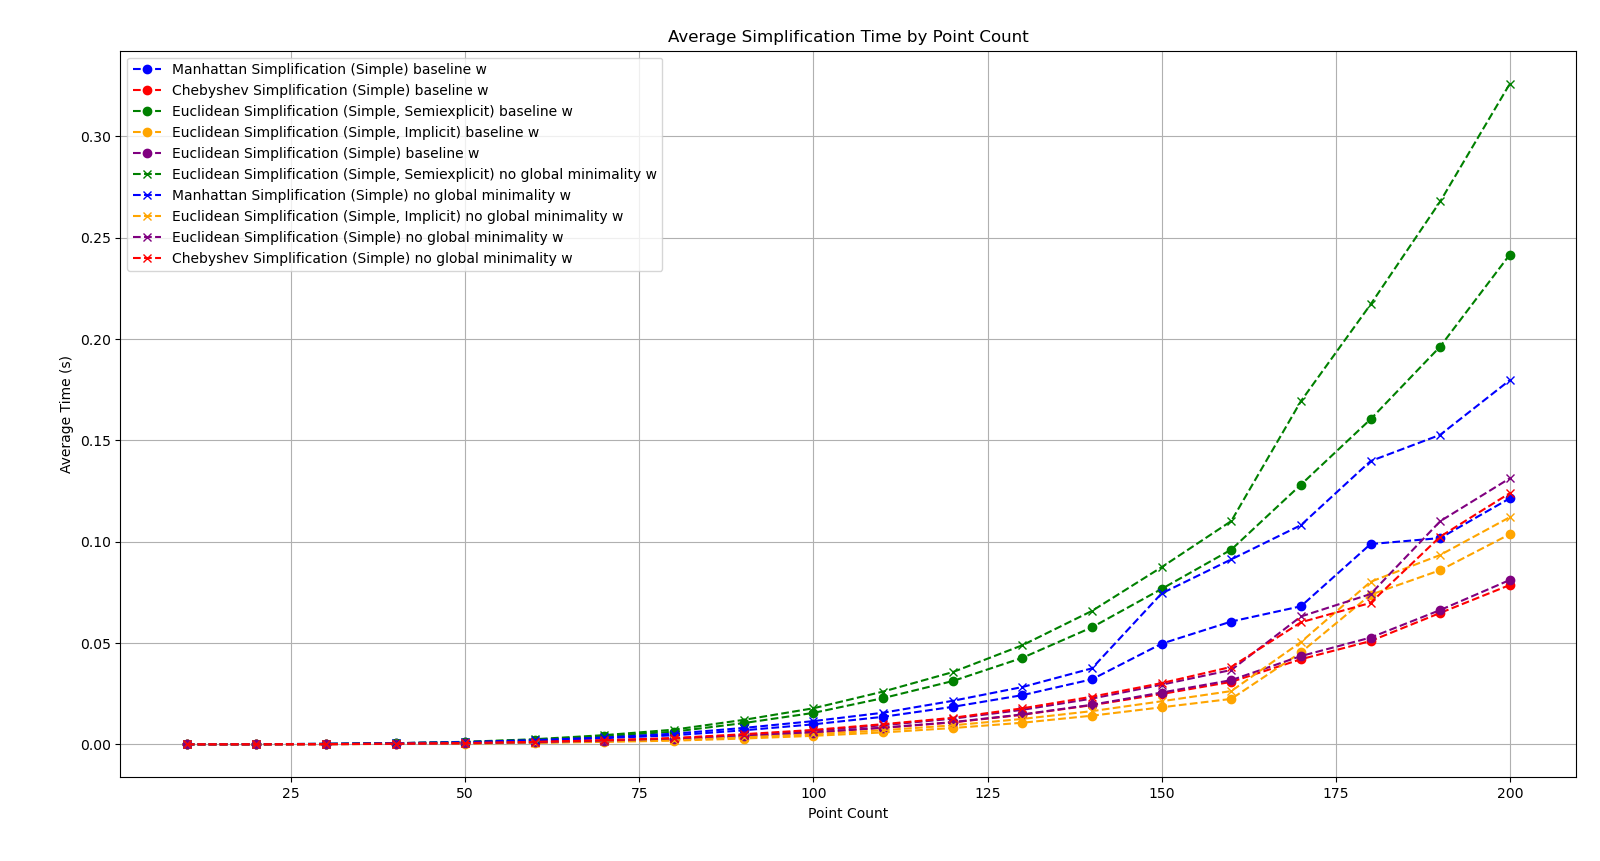
\includegraphics[scale=0.4]{./figures/simple-g.png}
  \caption{Simple algorithm with all optimizations and with all but the global optimality optimization.}
  \label{fig:simple-g}
\end{figure}

\begin{figure}[b]
  \centering
	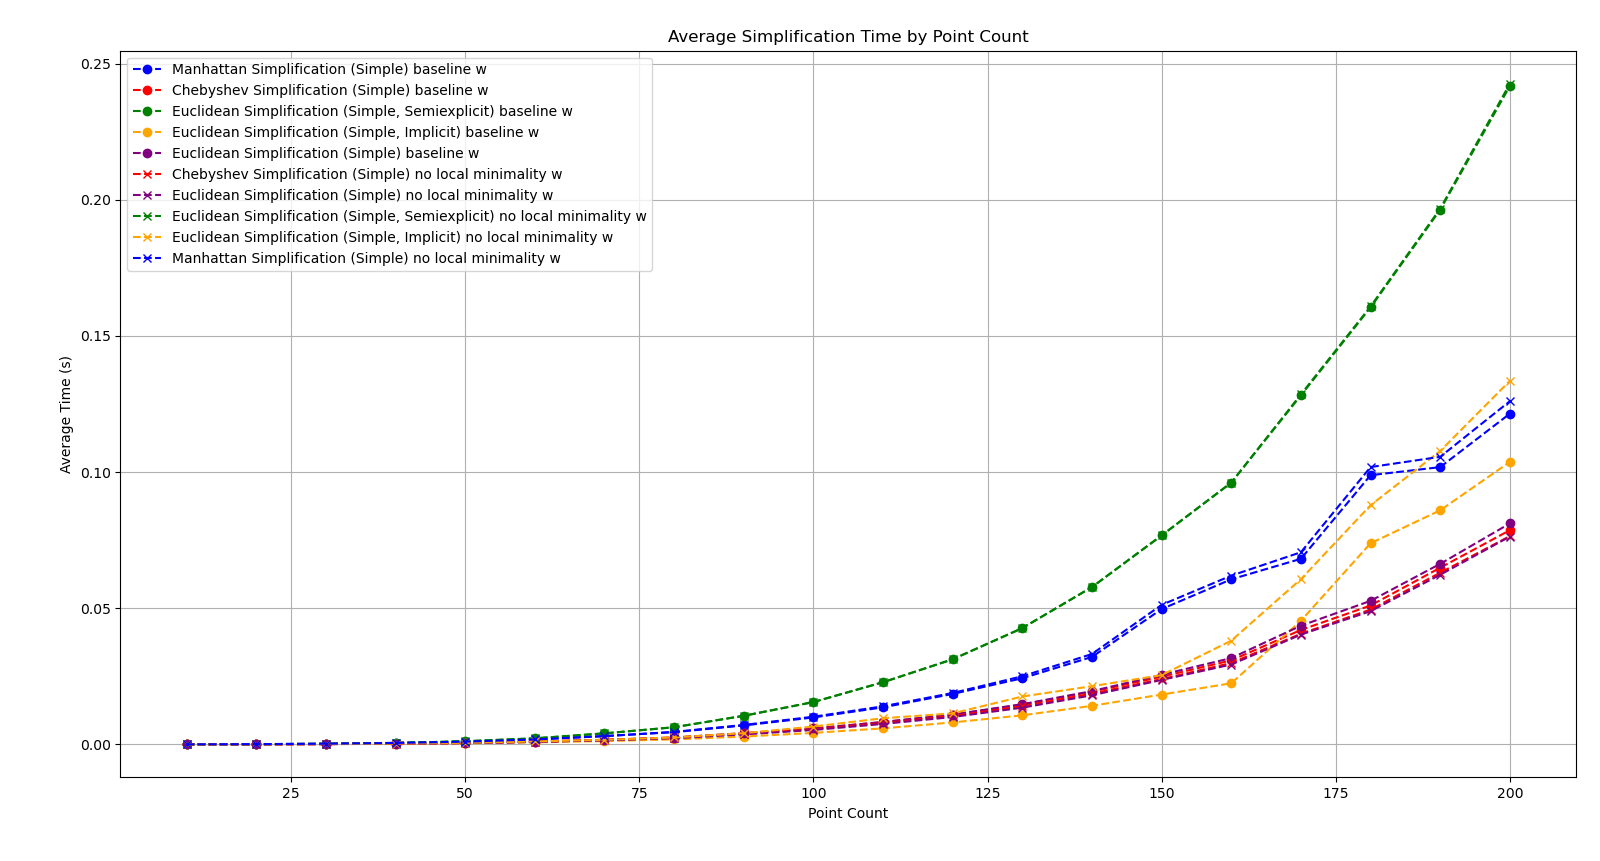
\includegraphics[scale=0.4]{./figures/simple-l.png}
  \caption{Simple algorithm with all optimizations and with all but the local optimality optimization.}
  \label{fig:simple-l}
\end{figure}

\begin{figure}[b]
  \centering
	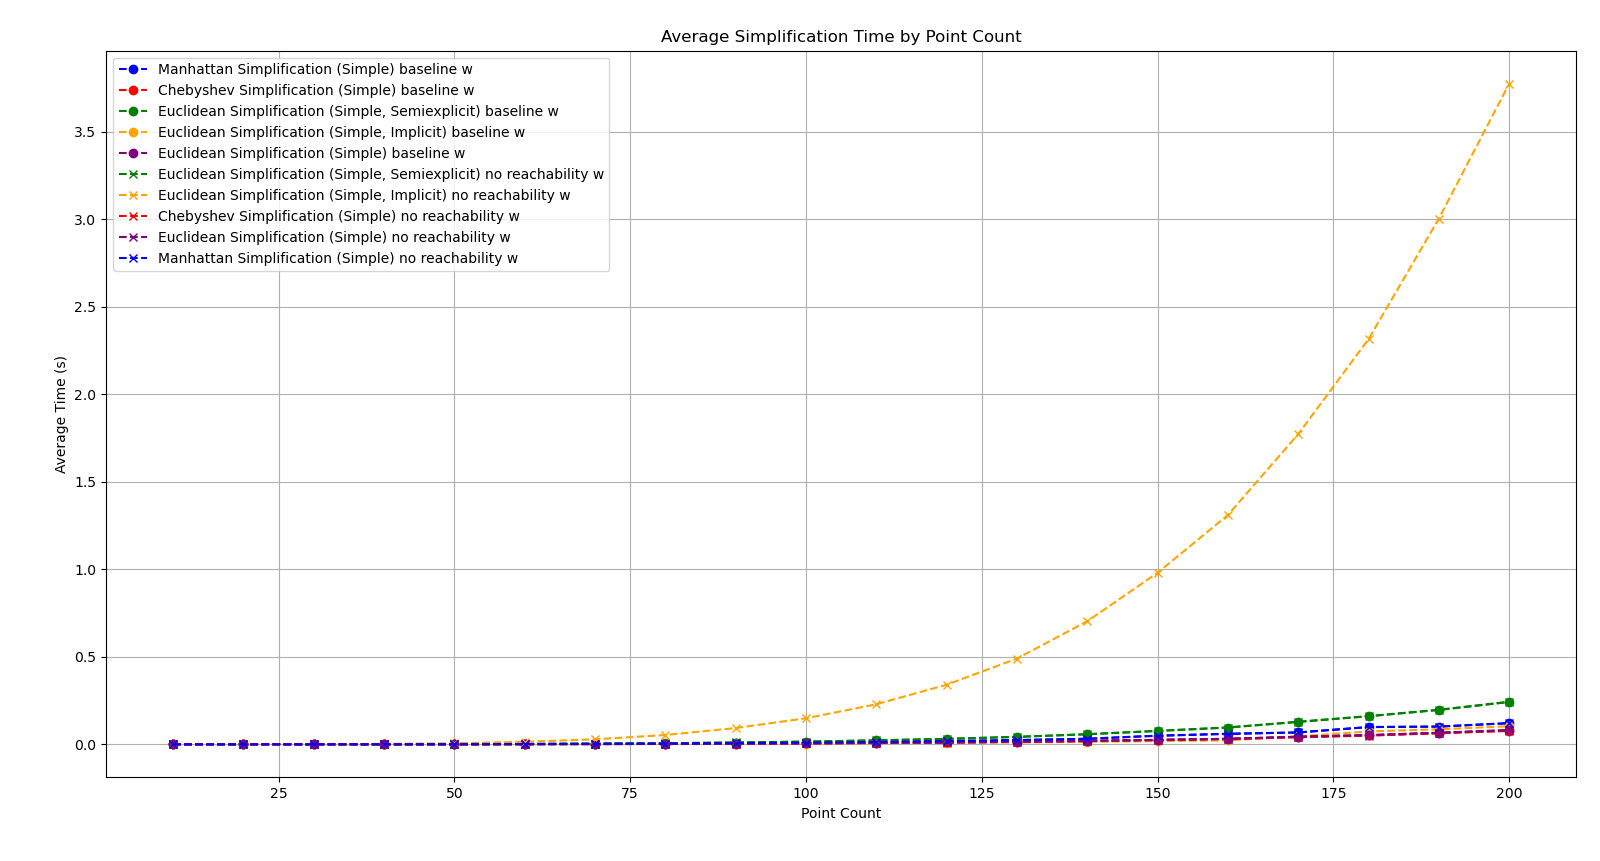
\includegraphics[scale=0.4]{./figures/simple-r.png}
  \caption{Simple algorithm with all optimizations and with all but the reachability optimization.}
  \label{fig:simple-r}
\end{figure}

\subsection{Results}
\label{subsec:results}

We present the results of our experimental evaluation in two parts. First, in \cref{ssubsec:runtime}, we perform a comprehensive analysis of the runtime performance of all nine algorithm variants. Second, in \cref{ssubsec:simplification_size}, we evaluate the quality of the simplifications by comparing their outputs.

\subsubsection{Runtime}
\label{ssubsec:runtime}

\Cref{fig:res_all300w} provides an overview of all nine variants on well-behaved data. The advanced versions are faster on longer polylines, while the simple variants remain competitive due to parallelization and the well-behaved nature of the input data. The semiexplicit Euclidean and Manhattan variants are the slowest in both the simple and advanced categories. For the simple variant, the semiexplicit version is by far the slowest, which we attribute to worse parallelizability caused by more complicated comparison operators. For the advanced versions, the Manhattan variant becomes the slowest, likely due to its more complex equation-solving algorithm, which cannot be offset by better parallelization.

\begin{figure}[b]
  \centering
	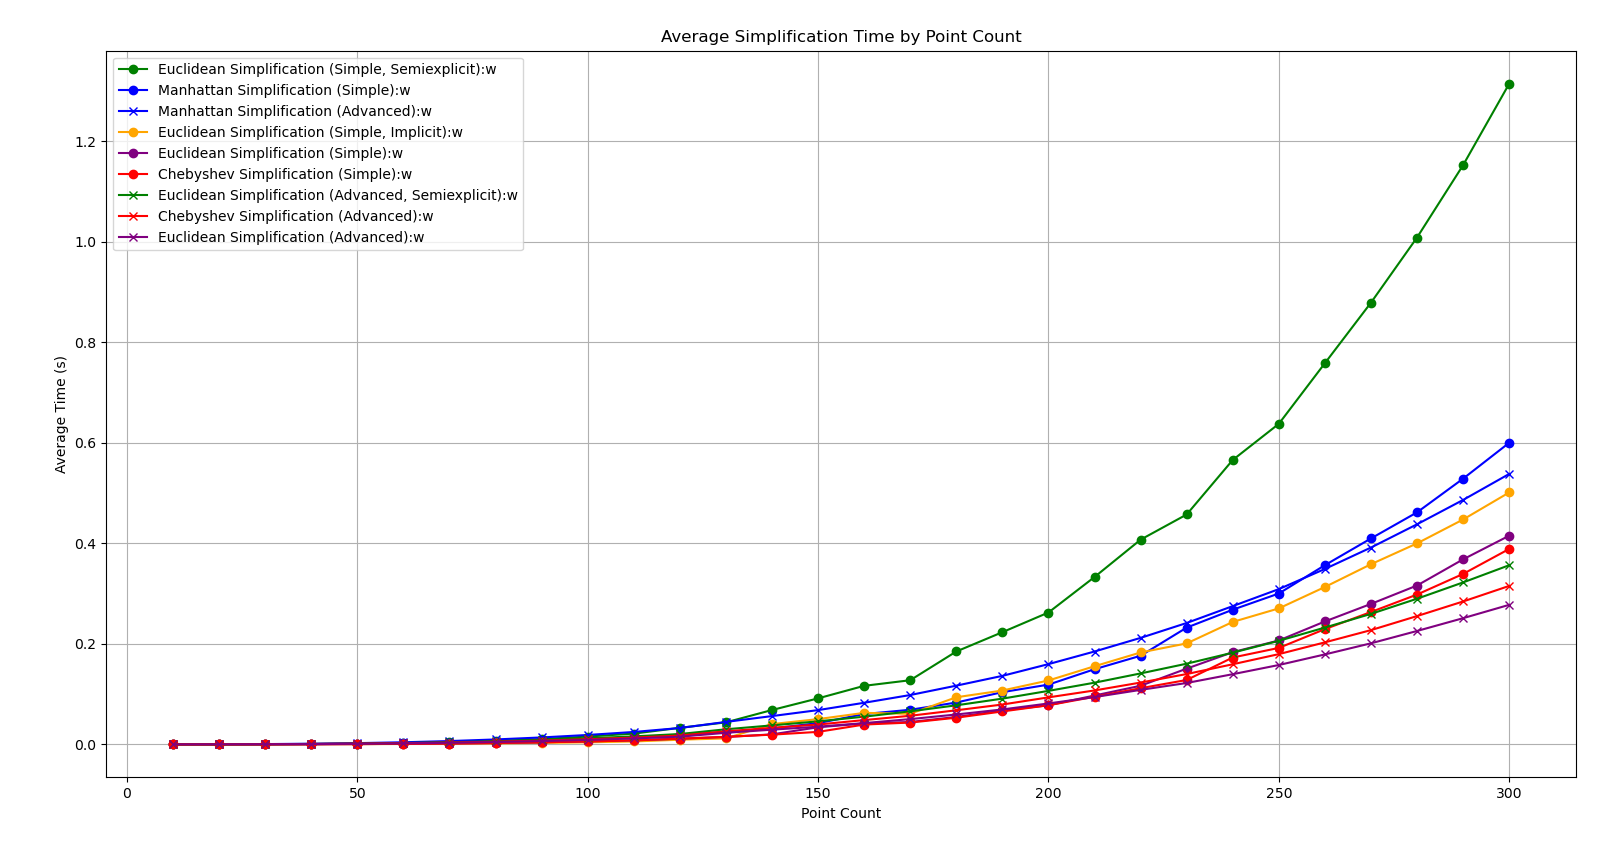
\includegraphics[scale=0.4]{figures/res_all300w.png}
  \caption{All nine variants on well-behaved data. Measurements are averages over 30 polylines per point count. Data marked with an ``x" are the advanced variants; those marked with dots are the simple variants.}
  \label{fig:res_all300w}
\end{figure}

It is notable that we were able to perform experiments on polylines of this size given the poor theoretical runtimes of \(\O(n^3)\) for the advanced and up to \(\O(n^6)\) for the simple algorithm\footnote{As shown in \cref{ssubsec:simplification_size}, the output sizes scale approximately linearly on the tested polylines, so the runtime of the simple algorithm is closer to \(\O(n^6)\) than \(\O(n^5)\).}. This can be explained by the fact that the individual operations are simple arithmetic operations that can be performed very quickly on modern hardware.

Furthermore, the stability of the data for the advanced variants is remarkable. The \citeauthor{polyline_simplification_has_cubic_complexity_bringmannetal} algorithm always performs the same computations regardless of the input polyline, but this degree of stability is surprising.

We extended the evaluation of the advanced variants to polylines of up to 800 points to gain further insights into their scaling. Given their observed stability, we reduced the test cases per polyline length to 2 to reduce total testing time. The results can be seen in \cref{fig:res_advanced800}. Even with more variance in individual data points, the trend remains stable and unsurprising. The variants are also insensitive to the well-behavedness of the data, as expected.

\begin{figure}[b]
  \centering
	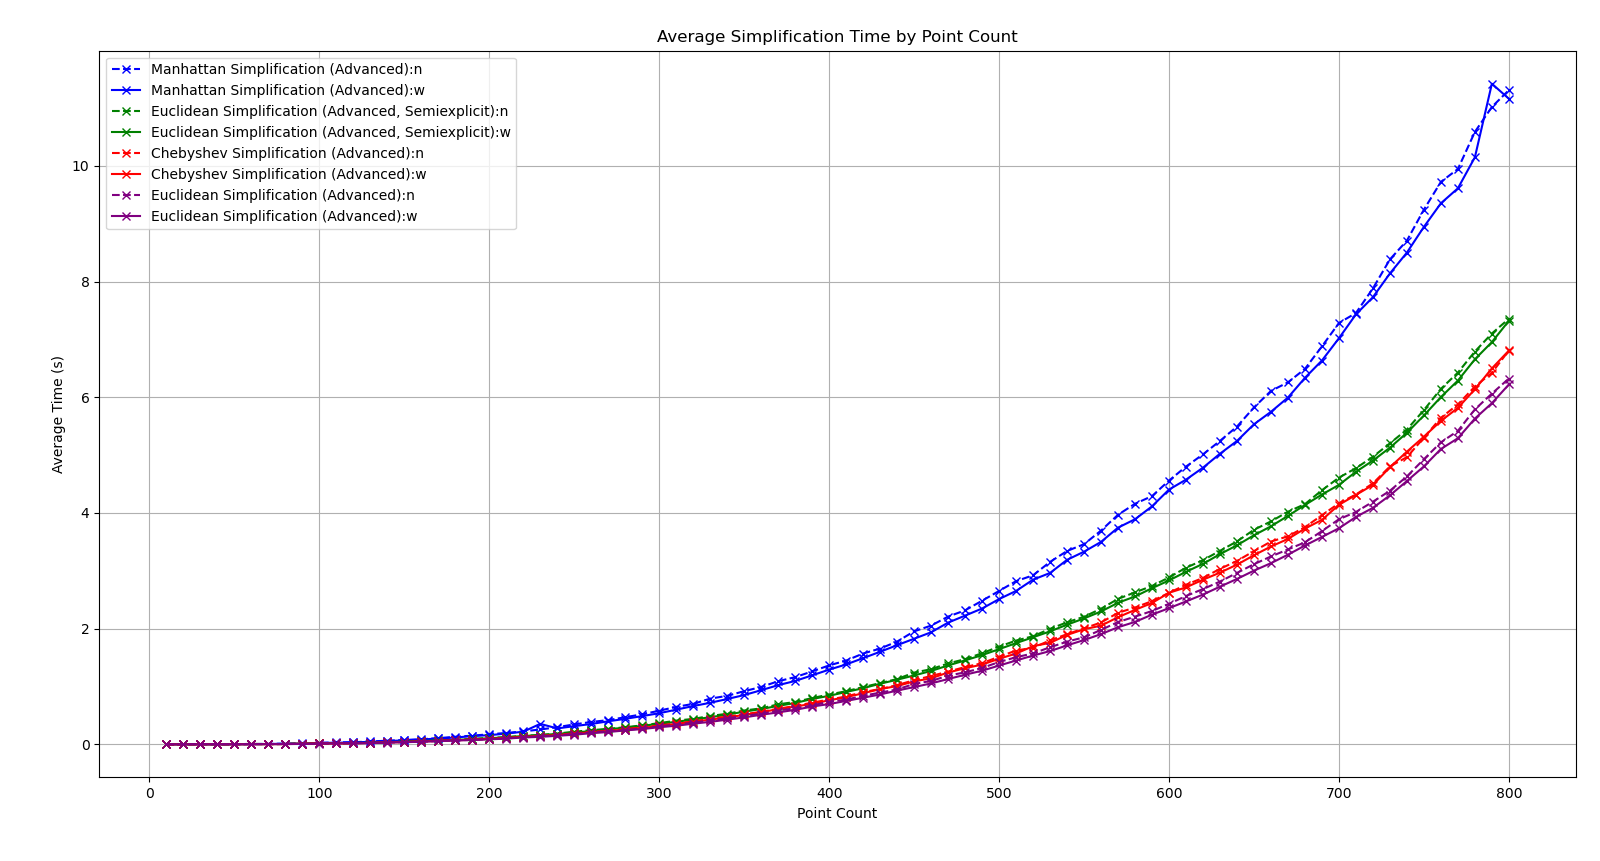
\includegraphics[scale=0.4]{./figures/res_advanced800.png}
  \caption{All advanced variants on well-behaved and non-well-behaved data. This uses only two cases per polyline size.}
  \label{fig:res_advanced800}
\end{figure}

We were not able to test longer polylines because preliminary testing revealed that larger polylines require too much space to be simplified.

We now examine in more detail the dependence of the simple algorithm's runtime on the input data in \cref{fig:res_simple}. Ignoring the semiexplicit variant (the slowest), all variants on well-behaved polylines take less time than any variant on non-well-behaved data. Another interesting insight is that the runtimes are more consistent on well-behaved data, while there is more variance for non-well-behaved data.

\begin{figure}[b]
  \centering
	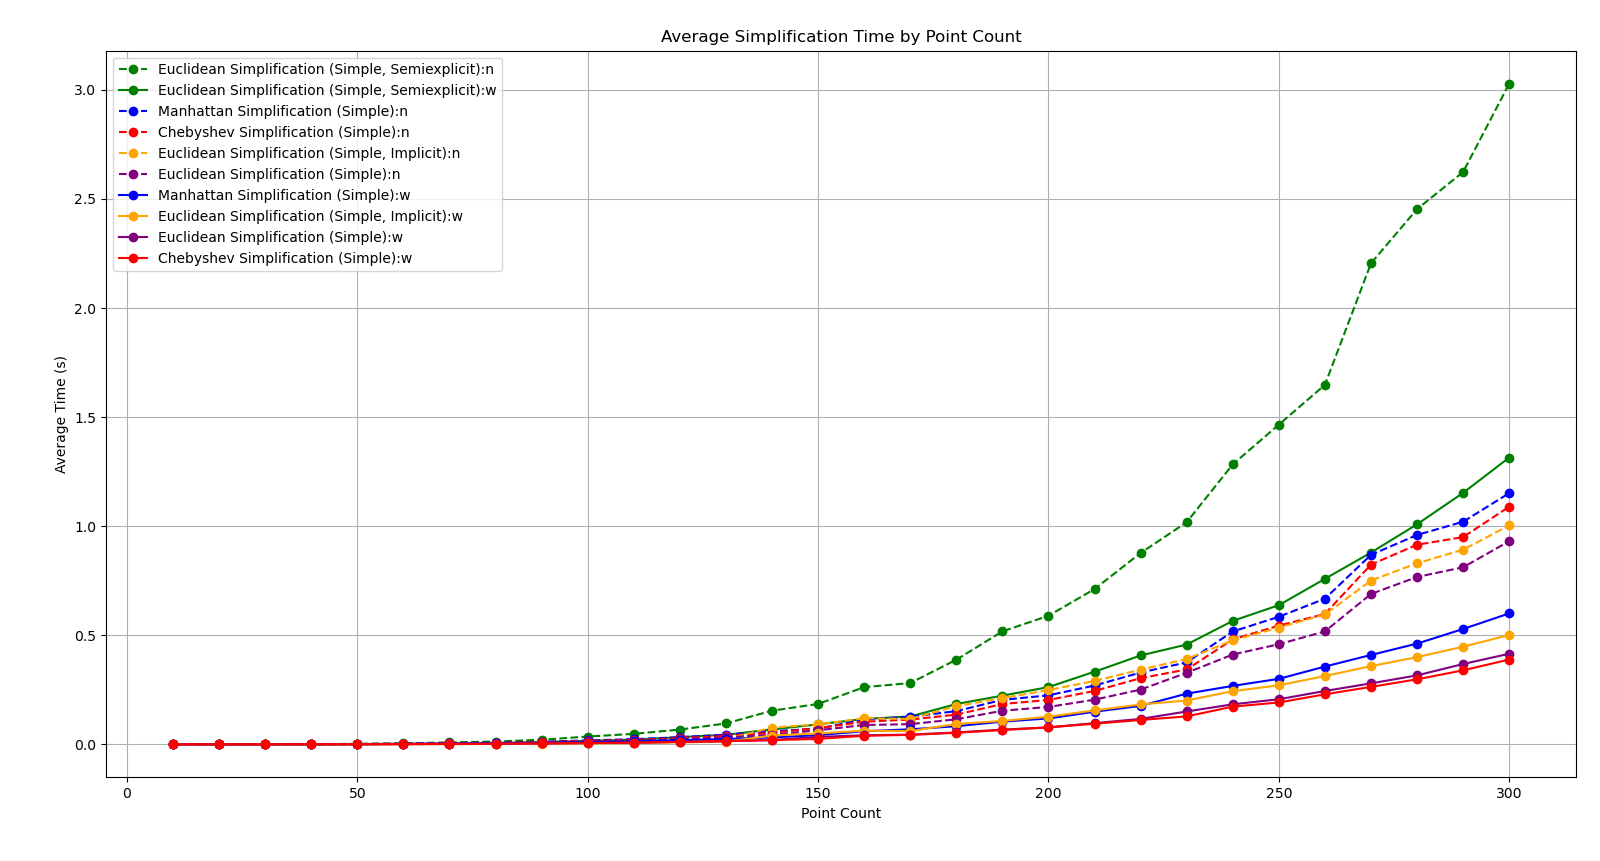
\includegraphics[scale=0.4]{./figures/res_simple.png}
  \caption{Effect of well-behavedness on the runtime of the simple algorithms.}
  \label{fig:res_simple}
\end{figure}

Finally, we show the runtime of the data structure construction algorithm (\cref{algo:query-datastructure}) in \cref{fig:res_ds}. We used only one test case per point count not only to reduce testing time but also to highlight the algorithm's stability. This notable stability can be explained by the predictable number of simplification calls required by the binary search and the already observed stability of the advanced algorithm used as a subroutine.

\begin{figure}[b]
  \centering
	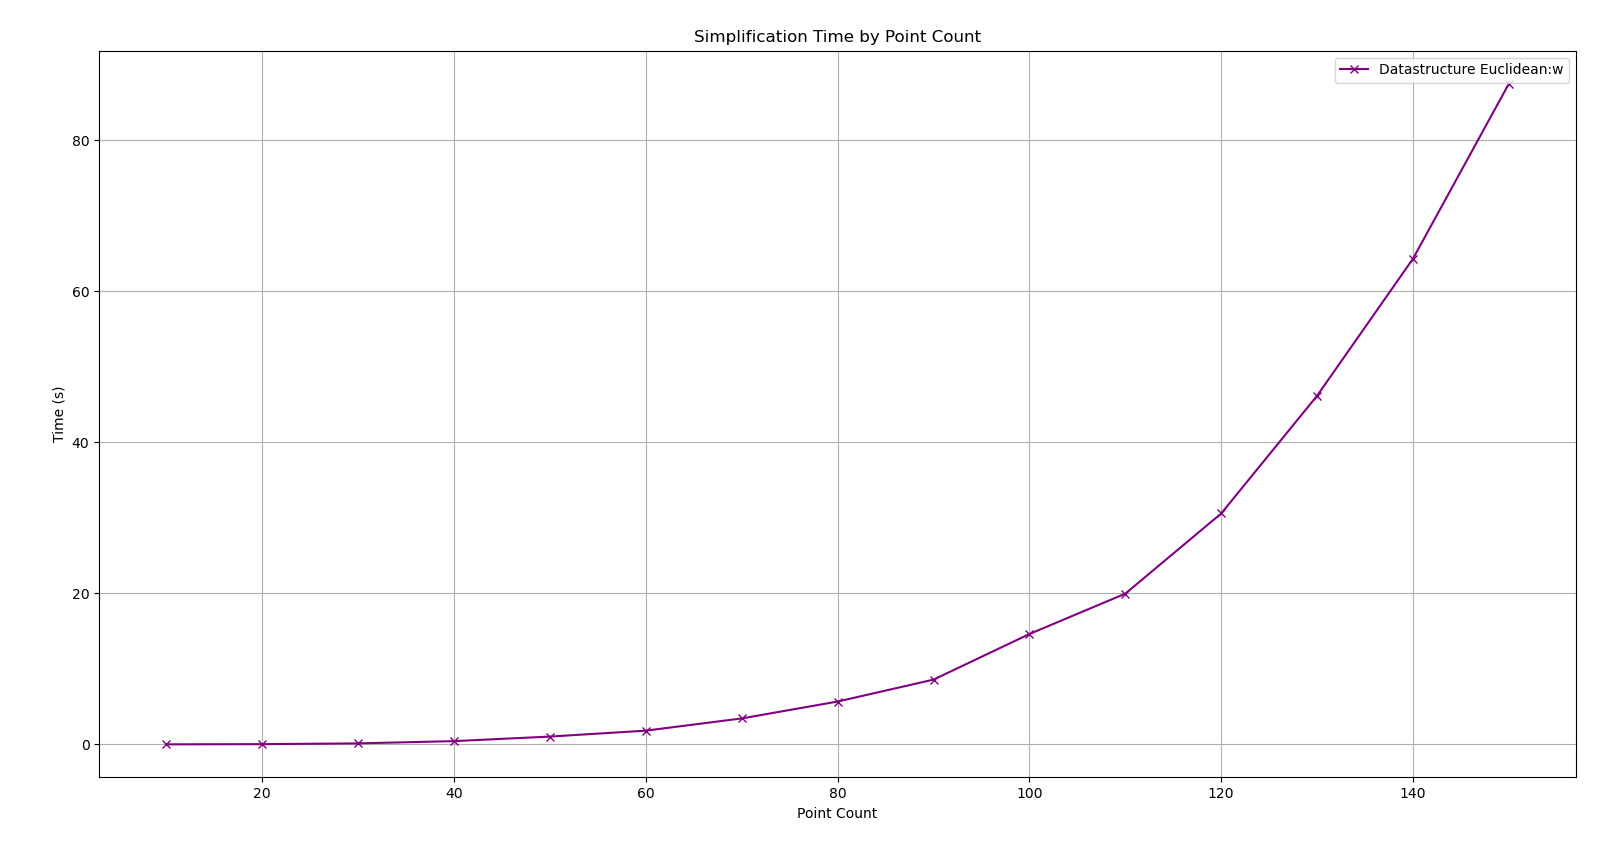
\includegraphics[scale=0.4]{./figures/res_ds.png}
  \caption{Runtime to create the data structure for simplification queries using the Euclidean distance, with one case per point count.}
  \label{fig:res_ds}
\end{figure}

\subsubsection{Simplification Size}
\label{ssubsec:simplification_size}
Having compared the performance of the algorithms, we now compare the simplifications and their sizes. This is independent of the algorithm used and depends only on the distance function, input data, and \(\varepsilon\).

\Cref{fig:simplification_sizes} shows the average computed sizes for the same data used in \cref{fig:res_all300w} and \cref{fig:res_simple}. It is clear that the Chebyshev simplifications are the smallest and the Manhattan ones are the largest, which we already know from \cref{cor:size_monotonicity}. However, the well-behavedness of the data has a greater impact on the size than the distance function used. The difference between the well-behaved Manhattan and the non-well-behaved Chebyshev simplifications is larger than the difference between the non-well-behaved or the well-behaved simplifications for the same distance. Other Minkowski distances \(\delta_\ell\) would fall between the Euclidean and Chebyshev distances if \(\ell > 2\), or between the Euclidean and Manhattan distances if \(\ell \in (1,2)\), so they would not create more spread within these well-behavedness clusters.

\begin{figure}[b]
  \centering
	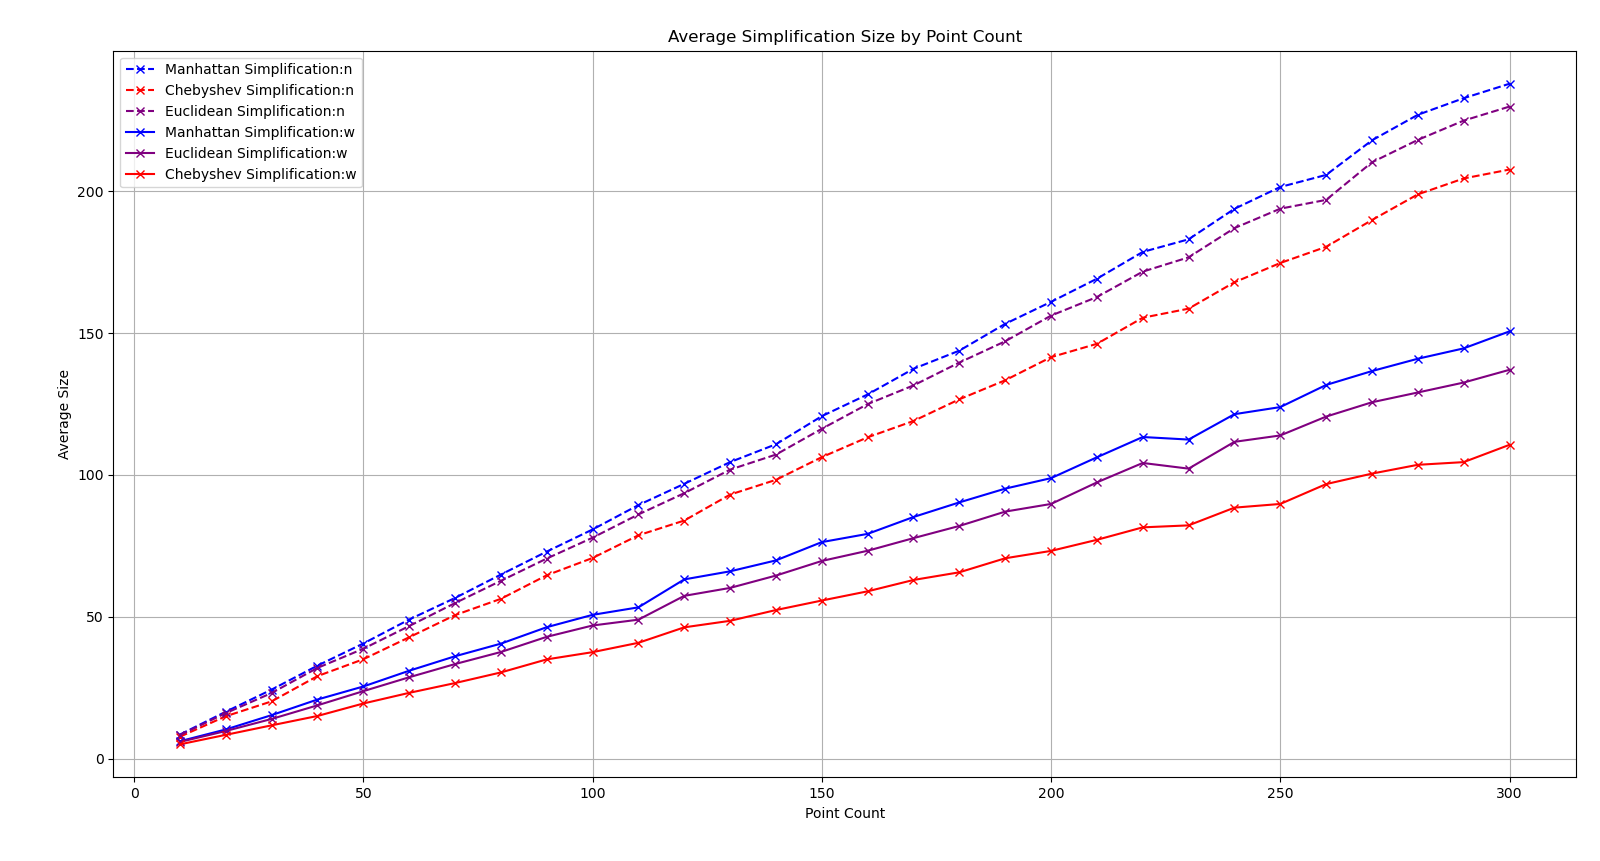
\includegraphics[scale=0.4]{./figures/simplification_sizes.png}
  \caption{Average simplification sizes of the tested data.}
  \label{fig:simplification_sizes}
\end{figure}

Next, we investigate the effect of \(\varepsilon\) on the simplification size in \cref{fig:vary_e10} and \cref{fig:vary_e200}. For this, we computed all intervals and resulting simplification sizes using the algorithm from \cref{sec:simplification-queries}. We then normalized \(\varepsilon\) to the interval \([0, 1]\) by dividing by \(\delta^F(P, e)\) for each polyline \(P\), where \(e\) is the line segment from the first to the last point (i.e., the shortest possible simplification). Thus, for normalized \(\varepsilon > 1\), the simplification size is 2, which is not shown.

Again, we see a clear difference between well-behaved and non-well-behaved polylines. Both roughly resemble rectangular hyperbolas, with the well-behaved data noticeably closer to the axes, meaning a smaller \(\varepsilon\) suffices for a large point reduction. Furthermore, the non-well-behaved data looks less smooth, possibly due to greater variance.

Interestingly, all four plots seem to approach concave functions, for which we have no explanation.

\begin{figure}[b]
  \centering
	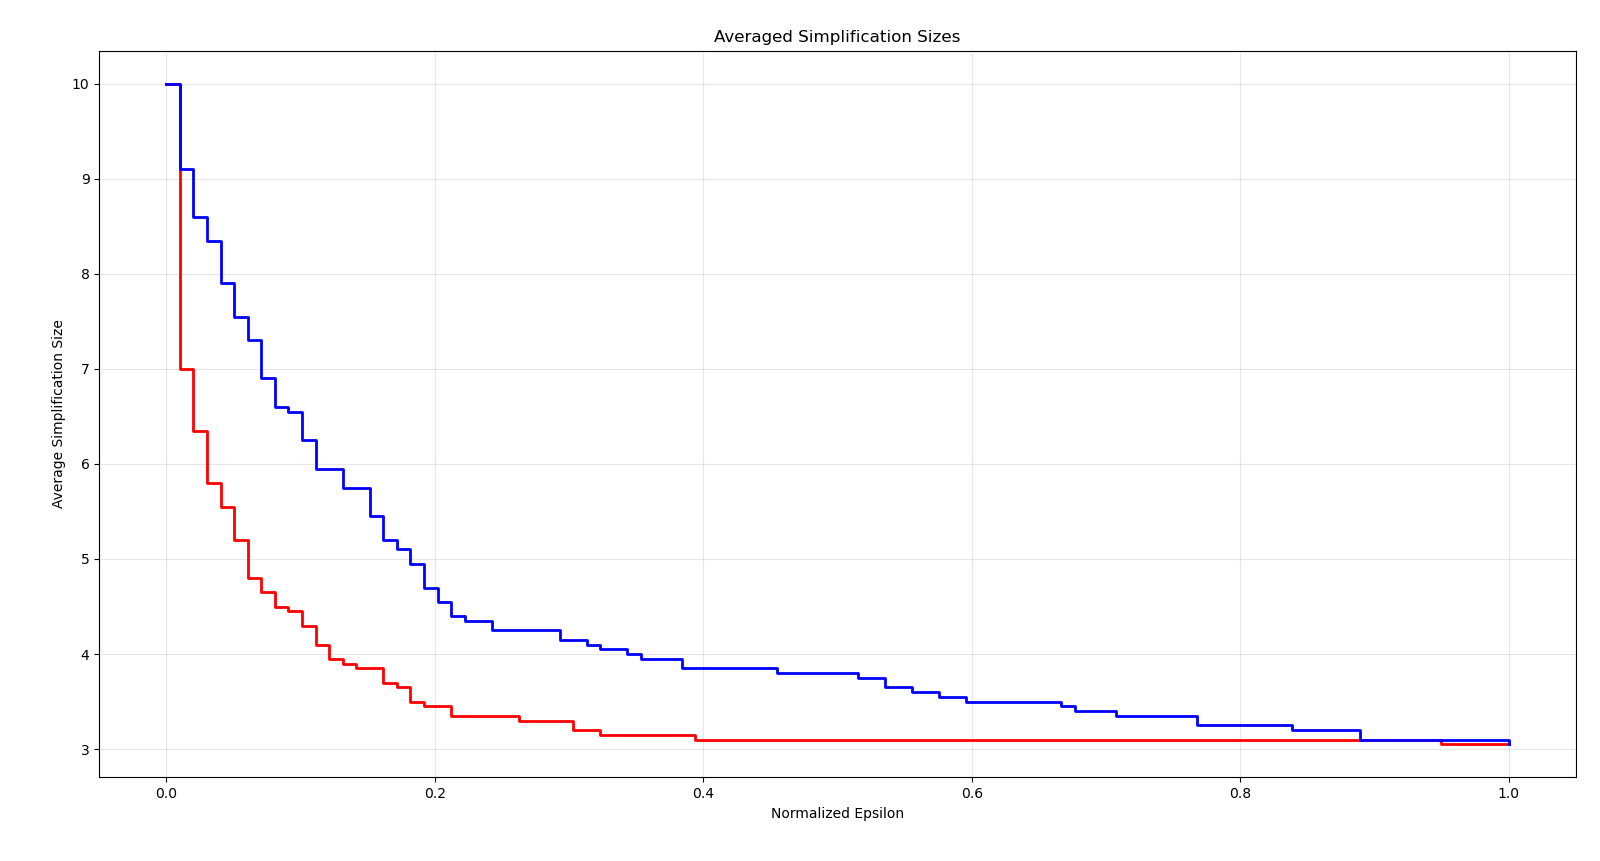
\includegraphics[scale=0.4]{./figures/vary_e10.png}
  \caption{Average simplification sizes of 20 polylines of length 10 over normalized \(\varepsilon\). Well-behaved in red and non-well-behaved in blue.}
  \label{fig:vary_e10}
\end{figure}

\begin{figure}[b]
  \centering
	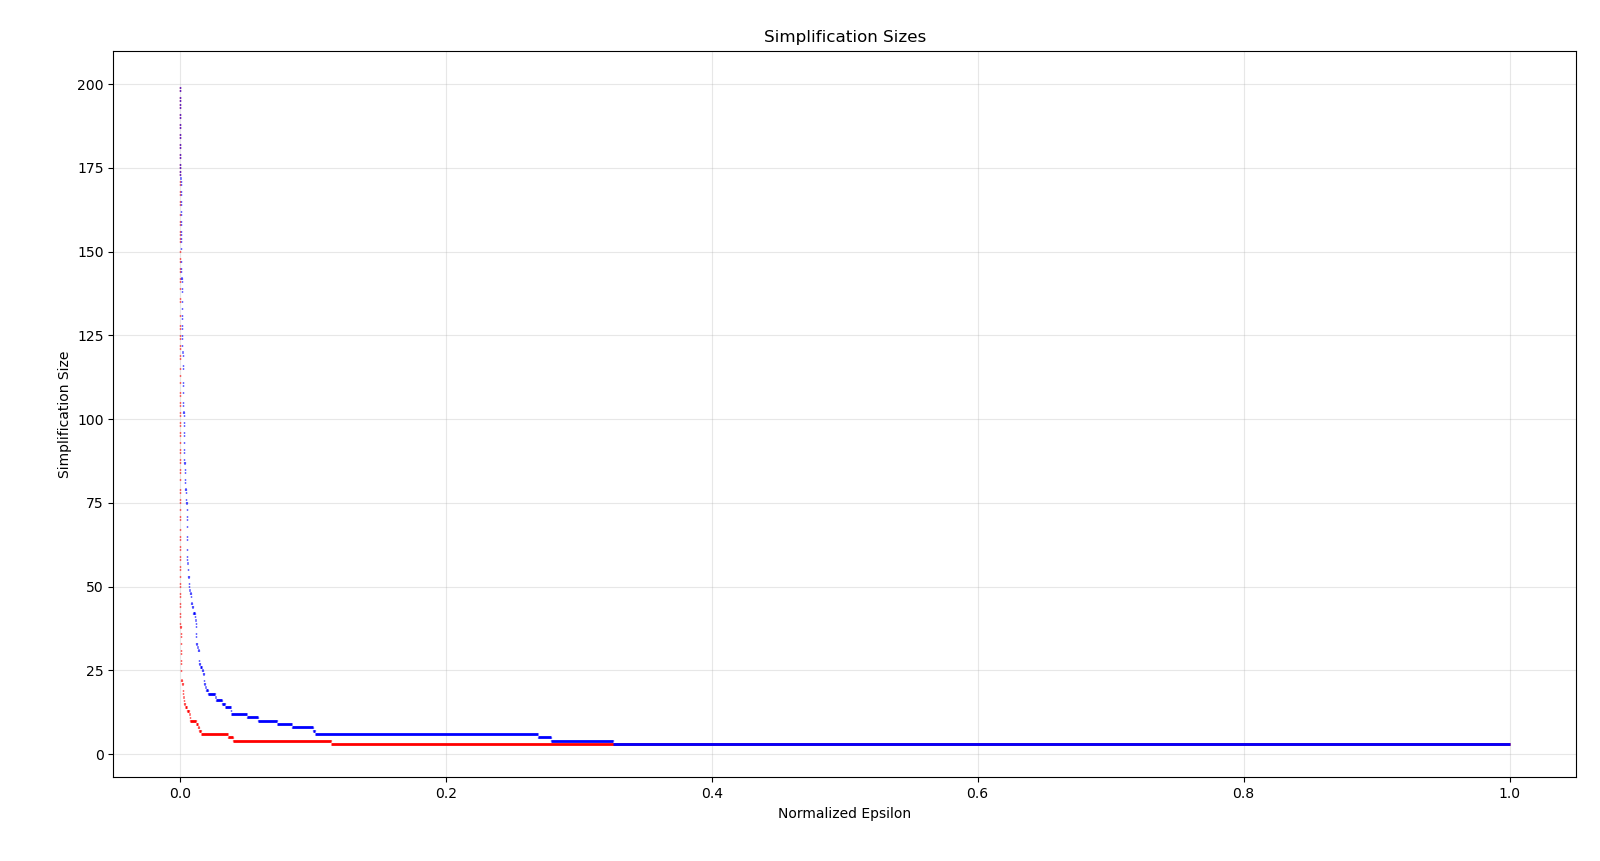
\includegraphics[scale=0.4]{./figures/vary_e200.png}
  \caption{Simplification sizes of a single polyline of length 200 over normalized \(\varepsilon\). Well-behaved in red and non-well-behaved in blue.}
  \label{fig:vary_e200}
\end{figure}

Finally, we investigate how local and global simplification sizes differ in \cref{fig:res-local-global}. For this, we used the Euclidean variant of the \citeauthor{computational_geometric_methods_for_polygonal_approximations_of_a_curve} algorithm (local Fréchet) for comparison and plotted the average simplification sizes on well-behaved and non-well-behaved data. This might be the most surprising result, as the sizes do not differ meaningfully. On well-behaved data, they are indistinguishable, and on non-well-behaved data, the local simplifications are only marginally larger.

\begin{figure}[b]
  \centering
	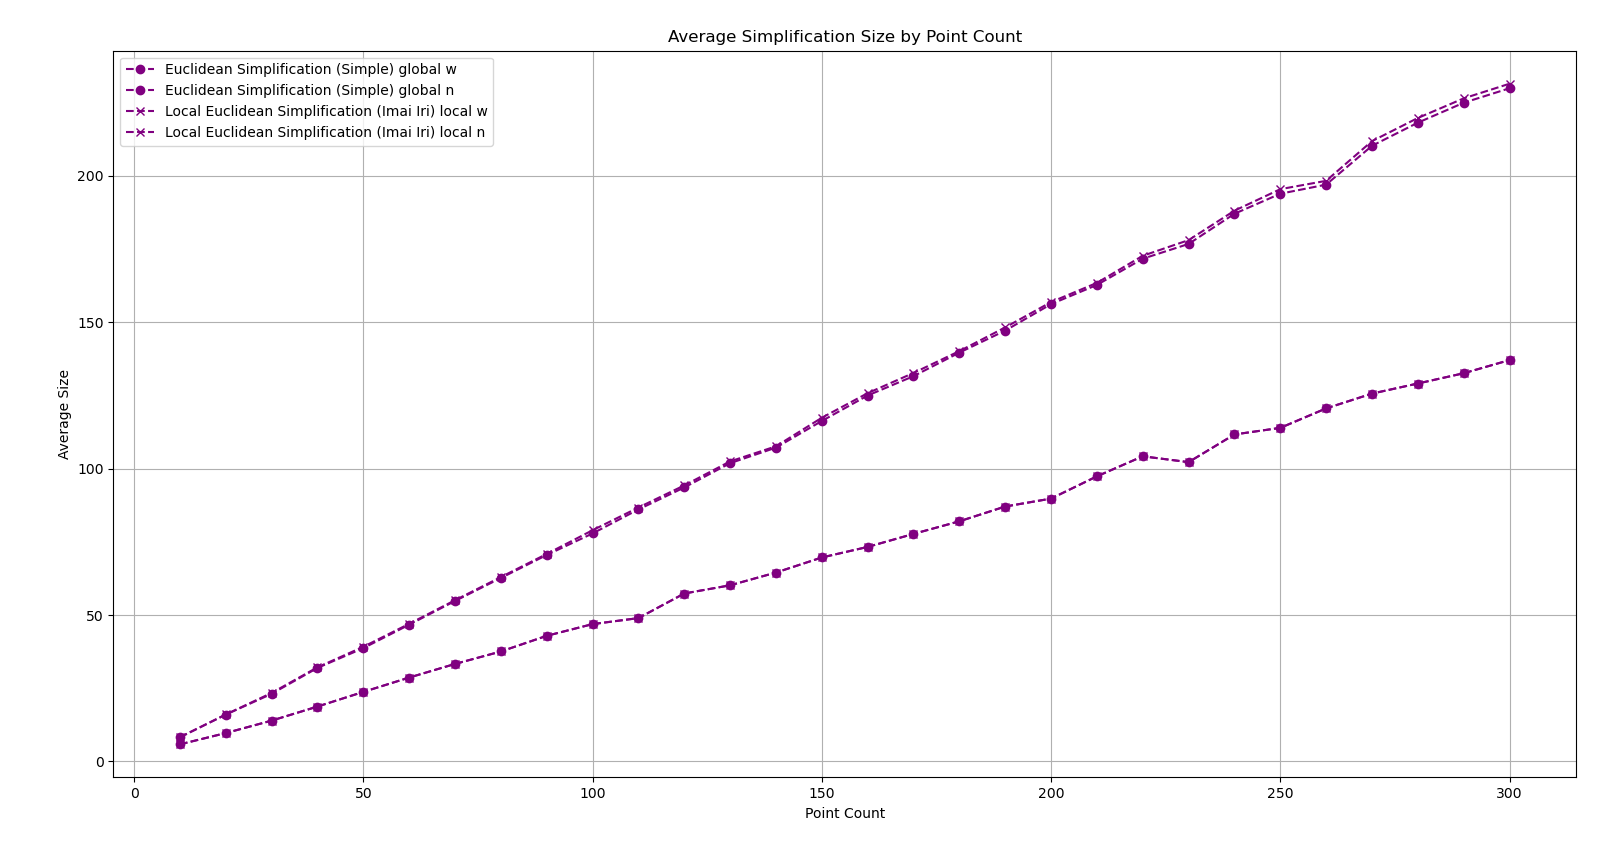
\includegraphics[scale=0.4]{./figures/res_local_global.png}
  \caption{Comparison of local and global simplification sizes on well-behaved and non-well-behaved data.}
  \label{fig:res-local-global}
\end{figure}

Given this result, we varied all parameters of our data generation method to try to find polylines and an \(\varepsilon\) where the local and global distances yield a large difference in simplification size. We chose random values for the minimum and maximum line segment length and the maximum angle. All tested polylines had 150 points in two dimensions. For each configuration, we repeatedly tested batches of 1000 polylines with a randomly generated \(\varepsilon\). The largest difference we encountered was 8, and the average difference over the 1000 iterations was never more than 0.3, meaning that on average there is no practical difference. This suggests that for all practical purposes, the global and local Fréchet distance yield similar simplification sizes and differ significantly only in degenerate, artificially crafted counterexamples.

Comparing our heuristic against the optimal simplification resulted in even less differences. While testing 500.000 polylines of length 100, we only found 8 with differing sizes. Only one of which had a resulted in a difference of two, the other ones differed only by one.
